\chapter{A Estrutura Hierárquica do BNDES}

Esta seção descreve e analisa de forma sucinta a estrutura hierárquica do \textbf{Banco Nacional de Desenvolvimento Econômico e Social} (BNDES), a partir do documento oficial de Organização Interna Básica (OIB) vigente em junho de 2026 \cite{bndes2026oib}. A análise discorrerá sobre quatro dimensões constitutivas de toda estrutura organizacional formal, a saber:

\begin{enumerate}
    \item o organograma organizacional;
    \item as linhas de comunicação;
    \item as unidades de trabalho; e
    \item a divisão horizontal do trabalho.
\end{enumerate}

De acordo com o relatório consultado, a estrutura hierárquica do BNDES caracteriza-se por uma organização formal, funcional e predominantemente vertical, combinada com mecanismos de articulação horizontal entre as diferentes unidades organizacionais.

\section{Organograma: representação gráfica da estrutura}

\begin{figure}[htb]
    \centering
    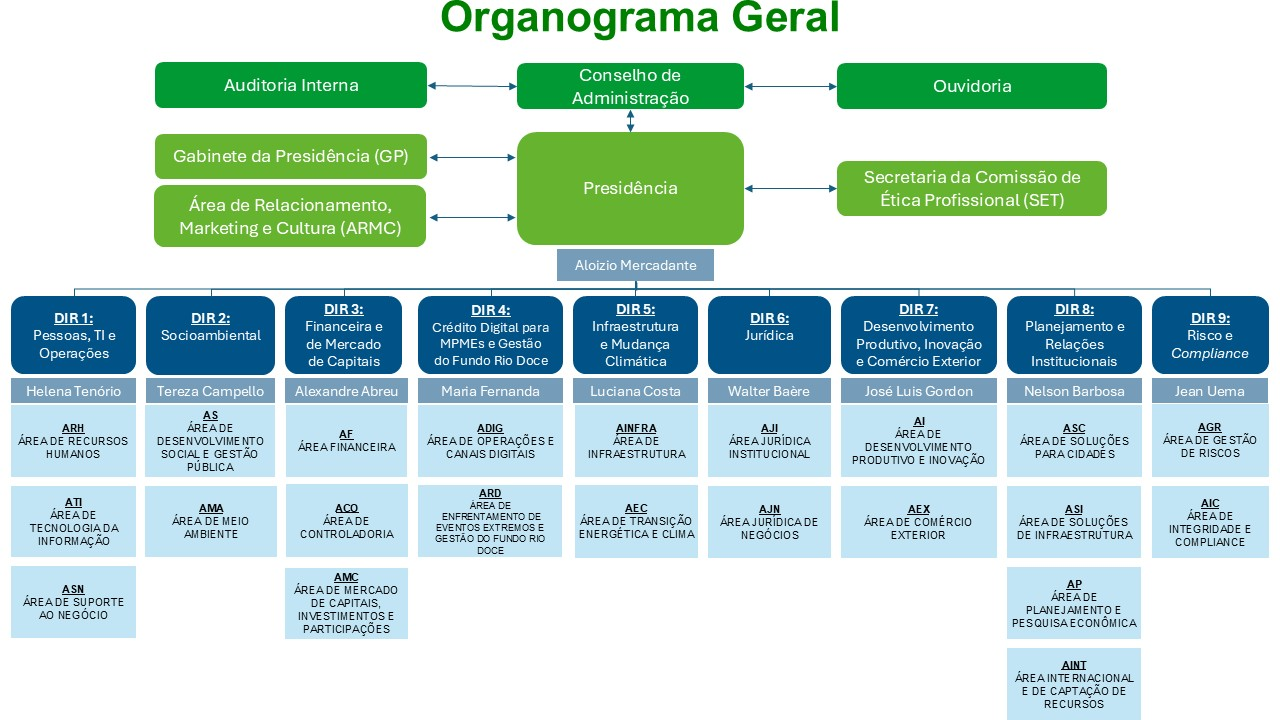
\includegraphics[
        width=\textwidth,
        keepaspectratio
    ]{img/cap_7/organograma_bndes}

    \caption{Organograma do BNDES.}
    \label{fig:organograma-bndes}

    \vspace{0.2cm}
    % \raggedright
    \footnotesize
    Fonte: BNDES (2026).
\end{figure}

% \section{Análise Descritiva da Estrutura organizacional}
% \subsection{Linhas de comunicação -- Formatos e modelos de comunicação interna}

% As linhas de comunicação representam os canais pelos quais informações, decisões, orientações, demandas e resultados circulam entre os diferentes níveis e unidades do BNDES.

% No modelo apresentado pelo documento, observa-se a existência de comunicação vertical \cite[p.~10]{bndes2026oib}, associada às relações de autoridade e subordinação, e de comunicação horizontal ou transversal, decorrente da necessidade de integração entre diferentes Unidades Fundamentais \cite[p.~11]{bndes2026oib}.

% A própria estrutura normativa estabelece que as unidades devem observar as políticas corporativas instituídas pelo Conselho de Administração e as normas operacionais aprovadas pela Diretoria Executiva. Também determina que as unidades planejem, organizem, coordenem e executem suas atividades de acordo com a autoridade superior à qual estão vinculadas.

% \subsection{Unidades de Trabalho -- Níveis de Autoridade}
% Elaborar


% \subsection{Hierarquia -- Cadeias de Comando e Tomada de Decisão}
% A estrutura de governança presente no órgão organiza-se de a partir de linhas claras de autoridade, separação de atribuições e competências deliberativas. Esta informação pode ser encontrada no Estatuto do BNDES \cite{brasil2002estatuto}. Destaca-se:

% \begin{enumerate}
%     \item \textbf{Conselho de Administração} -- constitui o órgão de orientação superior e deliberação estratégica do BNDES, integrando a cúspide da estrutura institucional de governança \cite[p.~24]{brasil2002estatuto}. Composto por conselheiros nomeados pelo Presidente da República e presidido por membro indicado pelo Ministério supervisor, o colegiado tem como núcleo de atuação fixar as diretrizes fundamentais de longo prazo, aprovar o Programa de Dispêndios Globais e apreciar as demonstrações financeiras e os relatórios anuais de auditoria \cite[p.~24]{brasil2002estatuto}. Compete privativamente a este conselho parametrizar os níveis de alçada decisória da Diretoria Colegiada e do Presidente para a aprovação formal de operações financeiras \cite[p.~24]{brasil2002estatuto}.
%     \item \textbf{Diretoria Colegiada} -- atua como o órgão executivo máximo de administração geral, sendo integrada pelo Presidente, pelo Vice-Presidente e por Diretores nomeados pelo Chefe do Poder Executivo Federal \cite[p.~26]{brasil2002estatuto}. É responsável por converter as diretrizes superiores em diretivas práticas de operação, podendo expedir normas e regulamentos de serviços, aprovar o orçamento gerencial e deliberar sobre o organograma interno e a respectiva distribuição de competências. No âmbito financeiro, é quem delibera conclusivamente acerca de operações de crédito cuja esfera financeira se situe na sua faixa de competência estabelecida pelo Conselho de Administração. O Presidente atua como líder da gestão executiva e representação externa do Banco, exercendo poder de veto sobre deliberações da Diretoria submetendo-as ao Conselho de Administração, além de deferir operações monocráticamente, quando aplicáveis \cite[p.~26--27]{brasil2002estatuto}.
%     \item \textbf{Comitês Internos e Instâncias Intermediárias} -- Destacam-se o Comitê de Crédito e Operações (CCOp) e o Comitê de Padronização de Procedimentos Jurídicos (CPPJ). Compete à Área de Gestão de Riscos (AGR) coordenar o CCOp e subsidiar a habilitação e elegibilidade de clientes e operações \cite[p.~35]{bndes2026oib}. Tais instâncias realizam a verificação cadastral, classificação de risco (rating), avaliação socioambiental e mitigação preventiva antes do trâmite às instâncias monocráticas ou executivas \cite[p.~21]{bndes2026oib}
% \end{enumerate}


% \subsection{Divisão Horizontal -- Identificação do Nível Hierárquico}
% Elaborar

\section{Detalhamento dos Componentes Estruturais}

\subsection{Hierarquia: Cadeias de Comando e Tomada de Decisão}

A cadeia de comando do BNDES está alicerçada em uma rígida segregação de competências deliberativas, normativas e executivas, concebida para assegurar conformidade legal, governança pública e sustentabilidade financeira \cite{bndes2025estatuto, bndes2026oib}:

\begin{enumerate}[label=\textbf{\alph*)}]
    \item \textbf{Conselho de Administração (Instância de Orientação e Deliberação Superior):} Composto por 11 (onze) membros eleitos pela Assembleia Geral \cite[art.~33]{bndes2025estatuto}, o Conselho de Administração é o órgão de deliberação máxima e orientação superior do Banco \cite[arts.~17,~I e 18]{bndes2025estatuto}. Compete privativamente ao colegiado:
          \begin{itemize}
              \item Fixar as diretrizes estratégicas, aprovar políticas institucionais (inclusive de governança, integridade, dividendos e pessoal) e subscrever a Carta Anual de Governança \cite[arts.~11 e 36,~VIII e IX]{bndes2025estatuto};
              \item Definir os níveis de alçada decisória para a Diretoria Executiva aprovar e conceder operações \cite[art.~43,~III]{bndes2025estatuto};
              \item Apreciar e manifestar-se sobre as demonstrações contábeis e a destinação de resultados propostas pela Diretoria Executiva, submetendo-as à deliberação da Assembleia Geral \cite[arts.~16,~I, 51,~II e 69]{bndes2025estatuto};
              \item Eleger e destituir os membros da Diretoria Executiva, bem como aprovar metas de gestão \cite[arts.~36,~VII e 39,~\S~1º]{bndes2025estatuto};
              \item Nomear e destituir o Ouvidor Geral, bem como aprovar a designação e destituição do titular da Auditoria Interna mediante proposta do Presidente do Banco \cite[art.~76]{bndes2025estatuto}, \cite[p.~11, itens II.2 e III.2]{bndes2026oib}.
          \end{itemize}
          Para resguardar sua independência, a \textbf{Auditoria Interna (AT)} vincula-se ao Conselho de Administração e ao Comitê de Auditoria \cite[arts.~52 e 57]{bndes2025estatuto}, \cite[p.~11, item II.2; p.~13]{bndes2026oib}. De igual modo, a \textbf{Ouvidoria} está vinculada diretamente ao CA, possuindo independência formal e mandato estrito de 36 meses para seu titular \cite[arts.~75 e 76]{bndes2025estatuto}, \cite[p.~11, item II.5; p.~27]{bndes2026oib}.

    \item \textbf{Diretoria Executiva (Gestão Executiva Superior e Alçadas de Crédito):} Órgão executivo de administração e representação composto pelo Presidente e por 9 (nove) Diretores Executivos eleitos pelo CA \cite[arts.~38 e 39]{bndes2025estatuto}. Possui competência originária para:
          \begin{itemize}
              \item Aprovar a estrutura organizacional e a respectiva distribuição de competências das áreas, mediante proposta do Presidente do Banco \cite[art.~78]{bndes2025estatuto}, \cite[p.~11, itens II.3 e II.4]{bndes2026oib};
              \item Aprovar as linhas orientadoras da ação do BNDES, as normas de operações e as normas de administração mediante regulamentos específicos \cite[art.~43,~II]{bndes2025estatuto};
              \item Deliberar colegiadamente sobre operações financeiras e limites operacionais, observados os limites de alçada estabelecidos pelo Conselho de Administração, sendo permitida a delegação para instâncias executivas no âmbito dos parâmetros normativos internos \cite[art.~43,~III e Parágrafo Único,~I]{bndes2025estatuto};
              \item Fixar limites operacionais e percentuais máximos de participação financeira para programas ou projetos específicos \cite[art.~7º,~Parágrafo Único]{bndes2025estatuto}.
          \end{itemize}
          As deliberações da Diretoria Executiva exigem registro formal em ata com justificativa de dissidências, cabendo ao Presidente a coordenação dos trabalhos, a representação institucional e a faculdade legal de veto submetido ao Conselho de Administração \cite[arts.~40 e 42]{bndes2025estatuto}.

    \item \textbf{Comitês Estatutários de Assessoramento e Comitês Internos:} O arcabouço decisório é apoiado por comitês estatutários obrigatórios previstos na Lei nº 13.303/2016 e pelo Estatuto Social:
          \begin{itemize}
              \item \emph{Comitê de Auditoria:} Vinculado ao CA, atua no monitoramento da integridade contábil, dos controles internos, da Ouvidoria e da Auditoria Interna \cite[arts.~52, 53 e 57]{bndes2025estatuto};
              \item \emph{Comitê de Riscos:} Avalia os limites regulatórios, o apetite institucional e a solvência das operações \cite[arts.~17,~VI e 61]{bndes2025estatuto};
              \item \emph{Comitê de Pessoas, Elegibilidade, Sucessão e Remuneração:} Valida requisitos cadastrais e legais de dirigentes e conselheiros \cite[arts.~21, 59 e 60]{bndes2025estatuto};
              \item \emph{Comitês Operacionais de Apoio:} Colegiados técnicos como o Comitê de Crédito e Operações (CCOp) e o Comitê de Padronização de Procedimentos Jurídicos (CPPJ), atuando na triagem e precificação prévia \cite[p.~21, 35, 163, 172]{bndes2026oib}.
          \end{itemize}

    \item \textbf{Rito de Tramitação Vertical de Financiamentos:} A deliberação sobre apoio financeiro segue um fluxo ascendente mandatório:
          \begin{enumerate}[label=\arabic*.]
              \item \emph{Ingresso e Triagem de Conformidade:} Habilitação cadastral, integridade de contraparte e conformidade regulatória conduzidas pela Área de Integridade e Compliance (AIC) \cite[arts.~7º,~III e 74,~IX e XI]{bndes2025estatuto}, \cite[p.~21, alínea ``q'']{bndes2026oib};
              \item \emph{Instrução Técnica Multidisciplinar:} Análise de viabilidade técnico-econômica, capacidade de pagamento e avaliação de implicações sociais e ambientais realizada pelos Departamentos e Gerências das Áreas operacionais \cite[art.~7º,~I]{bndes2025estatuto}, \cite[p.~45, 63]{bndes2026oib};
              \item \emph{Avaliação de Riscos e Chancelas Jurídicas:} Mensuração do risco de crédito de contraparte pela Área de Gestão de Riscos (AGR) \cite[art.~74]{bndes2025estatuto}, \cite[p.~35, 138]{bndes2026oib} e exame jurídico minucioso pela Área Jurídica de Negócios (AJN) \cite[p.~171--172]{bndes2026oib};
              \item \emph{Deliberação das Alçadas Competentes:} Apreciação pelos comitês intermediários e decisão no âmbito dos limites de alçada delegados ou homologação privativa pela Diretoria Executiva \cite[art.~43,~III e Parágrafo Único,~I]{bndes2025estatuto}.
          \end{enumerate}
\end{enumerate}

\subsection{Unidades de Trabalho: Níveis de Autoridade}

A arquitetura interna do BNDES é dividida em níveis hierárquicos e unidades de trabalho claramente escalonadas no Estatuto e no Caderno OIB \cite[art.~78]{bndes2025estatuto}, \cite[p.~11, item II.4]{bndes2026oib}:

\begin{itemize}
    \item \textbf{Superintendentes de Área (Unidades Fundamentais -- UFs):} Representam o escalão tático-estratégico que lidera as grandes áreas temáticas institucionais \cite[p.~10, item II.1]{bndes2026oib}. Respondem diretamente ao Presidente ou aos Diretores Executivos por delegação deste \cite[arts.~40 e 78]{bndes2025estatuto}, \cite[p.~11, item II.3]{bndes2026oib}. Sua designação e exoneração competem privativamente ao Presidente do Banco \cite[p.~11, item III.3]{bndes2026oib} -- ressalvado o titular da Auditoria Interna, cuja investidura é aprovada pelo Conselho de Administração \cite[p.~11, item III.2]{bndes2026oib}. O Superintendente detém autoridade para planejar, supervisionar orçamentos setoriais, despachar minutas executivas com a Diretoria Executiva e aprovar pareceres técnicos e jurídicos vinculantes no âmbito de sua competência \cite[p.~11, 45, 158, 172]{bndes2026oib}.

    \item \textbf{Chefes de Departamento (Unidades Administrativas Principais -- UAPs):} Constituem o escalão de gestão setorial especializada \cite[p.~11, item II.4]{bndes2026oib}. Exercem autoridade gerencial direta sobre carteiras temáticas. Têm autonomia delegada para coordenar a elaboração de notas e pareceres técnicos, subsídios a políticas públicas, gestão de riscos operacionais inerentes aos seus processos e instrução dos pleitos a serem submetidos às instâncias deliberativas \cite[p.~45, 63, 120, 147]{bndes2026oib}.

    \item \textbf{Gerentes Executivos e Gerentes Setoriais:} Nível de coordenação operacional e supervisão imediata das equipes técnicas de projeto \cite[p.~11, item II.4]{bndes2026oib}. \textbf{Princípio de Segregação Mandatória:} O Estatuto e o Caderno OIB prescrevem como diretriz estruturante que as Áreas e Departamentos Operacionais devem obrigatoriamente designar pelo menos uma gerência especializada exclusivamente no \emph{acompanhamento pós-contratação das operações}, segregando-a funcionalmente das gerências focadas na \emph{análise prévia e concessão de crédito} \cite[art.~74,~XI]{bndes2025estatuto}, \cite[p.~11, item II.7; p.~126]{bndes2026oib}. Essa segregação neutraliza potenciais conflitos de interesse na verificação das condições de eficácia e desembolso.

    \item \textbf{Equipes Técnicas Multidisciplinares (Corpo Técnico Funcional):} Compostas por empregados públicos admitidos mediante concurso público (CLT) \cite[art.~79]{bndes2025estatuto}, abrangendo economistas, contadores, engenheiros, advogados e administradores \cite[p.~11, item II.7; p.~45, 172]{bndes2026oib}. Possuem autonomia funcional para fundamentar notas técnicas, desenhar matrizes de mitigação de risco e atestar a aderência de engenharia e conformidade regulatória \cite[art.~7º,~I]{bndes2025estatuto}, \cite[p.~45, 172]{bndes2026oib}.
\end{itemize}

\subsection{Divisão Horizontal: Identificação do Nível Hierárquico e Especialização}

A distribuição horizontal do BNDES estrutura-se no nível das Unidades Fundamentais (UFs), situadas no mesmo patamar hierárquico sob a supervisão das Diretorias Executivas, aplicando os princípios de especialização técnica, complementaridade e controle mútuo \cite[art.~78]{bndes2025estatuto}, \cite[p.~10--11]{bndes2026oib}:

\begin{enumerate}[label=\textbf{\arabic*.}]
    \item \textbf{Diretorias e Áreas Finalísticas (Fomento e Concessão):} Especializam-se no atendimento setorial às prioridades da política de desenvolvimento e prestação de serviços econômico-financeiros de interesse público \cite[arts.~6º e 7º]{bndes2025estatuto}:
          \begin{itemize}
              \item \emph{Área de Desenvolvimento Produtivo e Inovação (AI):} Apoio ao complexo industrial, inovação e transição tecnológica \cite[p.~43, 45]{bndes2026oib};
              \item \emph{Área de Operações e Canais Digitais (ADIG):} Financiamento descentralizado e automático via rede credenciada de agentes financeiros e garantias de crédito \cite[p.~54, 63, 70]{bndes2026oib};
              \item \emph{Área de Soluções para Cidades, Gestão Pública e Social (ASC/AS):} Estruturação de parcerias de desestatização, infraestrutura urbana, saneamento e inclusão produtiva \cite[art.~6º,~XII e XIII]{bndes2025estatuto}, \cite[p.~87, 118, 120]{bndes2026oib};
              \item \emph{Área de Mercado de Capitais, Investimentos e Participações (AMC):} Subscrição de títulos mobiliários, renda variável e fundos de investimento \cite[art.~43,~III, ``f'']{bndes2025estatuto}, \cite[p.~99--106]{bndes2026oib};
              \item \emph{Área de Comércio Exterior e Área Internacional e de Captação (AINT):} Apoio à exportação e captação de recursos junto a organismos multilaterais \cite[p.~10, 107--113]{bndes2026oib};
              \item \emph{Área de Transição Energética e Climática (AEC):} Fomento à descarbonização, energias renováveis e projetos de combate à mudança climática \cite[art.~6º,~X, ``b'']{bndes2025estatuto}, \cite[p.~111--112]{bndes2026oib}.
          \end{itemize}

    \item \textbf{Diretorias e Áreas Instrumentais, de Controle e Suporte (Gestão Institucional):}
          \begin{itemize}
              \item \emph{Área de Gestão de Riscos (AGR):} Mensuração e controle prudencial dos riscos de crédito, mercado, liquidez, modelo e risco operacional corporativo \cite[art.~74]{bndes2025estatuto}, \cite[p.~35, 138]{bndes2026oib};
              \item \emph{Área de Integridade e Compliance (AIC) e Corregedoria:} Promoção de conformidade, programas anticorrupção, verificação de \emph{background check} e gestão de integridade institucional com independência funcional \cite[arts.~73,~\S~3º e 74]{bndes2025estatuto}, \cite[p.~11, item II.8; p.~21, 29, 33]{bndes2026oib};
              \item \emph{Área de Controladoria (ACO):} Demonstrações financeiras, registros contábeis societários e aderência às regras do CMN \cite[art.~80]{bndes2025estatuto}, \cite[p.~35, 38]{bndes2026oib};
              \item \emph{Áreas Jurídicas Segregadas:} O BNDES adota especialização técnica entre a \textbf{Área Jurídica Institucional (AJI)}, encarregada de governança societária, órgãos colegiados e contencioso judicial \cite[p.~148, 163]{bndes2026oib}, e a \textbf{Área Jurídica de Negócios (AJN)}, focada na estruturação de contratos de financiamento, garantias e captação externa \cite[p.~171--172]{bndes2026oib};
              \item \emph{Área de Recursos Humanos (ARH)}, \emph{Tecnologia da Informação (ATI)} e \emph{Suporte ao Negócio (ASN)}: Gestão de pessoas, suporte logístico e sustentação tecnológica \cite[p.~11, 73, 133, 147]{bndes2026oib}.
          \end{itemize}

    \item \textbf{Interdependência no Modelo das Linhas de Defesa:} A cooperação entre as unidades opera de forma cruzada segundo as diretrizes estatutárias e de governança pública:
          \begin{itemize}
              \item \emph{1ª Linha de Defesa (Unidades Finalísticas Operacionais):} Gerenciam os riscos operacionais e creditícios na sua gênese durante o enquadramento, estruturação e acompanhamento físico-financeiro \cite[art.~7º,~I]{bndes2025estatuto}, \cite[p.~45, 63]{bndes2026oib};
              \item \emph{2ª Linha de Defesa (AGR, AIC, ACO e Áreas Jurídicas):} Estabelecem metodologias, monitoram limites, asseguram a conformidade normativa e fiscalizam o princípio de segregação de funções com independência assegurada \cite[arts.~73,~\S~3º e 74]{bndes2025estatuto}, \cite[p.~21, 33, 35, 172]{bndes2026oib};
              \item \emph{3ª Linha de Defesa (Auditoria Interna -- AT):} Avalia de maneira objetiva e independente a integridade das 1ª e 2ª linhas, subordinada hierarquicamente ao Conselho de Administração \cite[arts.~52 e 57]{bndes2025estatuto}, \cite[p.~11, item II.2; p.~13]{bndes2026oib}.
          \end{itemize}
\end{enumerate}

\subsection{Linhas de Comunicação: Formatos e Modelos de Comunicação Interna}

A formalização da comunicação no BNDES é estritamente regulamentada para assegurar conformidade com as normas da administração pública e mitigar riscos institucionais \cite{bndes2025estatuto, bndes2026oib}:

\begin{itemize}
    \item \textbf{Comunicação Descendente (Fluxo Top-Down -- Normatização e Comando):}
          \begin{itemize}
              \item \emph{Resoluções da Diretoria Executiva:} Instrumentos deliberativos normativos que aprovam políticas corporativas, quadros funcionais, orçamentos e regulamentos específicos de operação \cite[arts.~43,~II e 78]{bndes2025estatuto}, \cite[p.~11]{bndes2026oib};
              \item \emph{Circulares e Ordens de Serviço:} Atos emitidos para uniformizar procedimentos entre departamentos e orientar os agentes financeiros credenciados \cite[p.~44, 172]{bndes2026oib};
              \item \emph{Canais Corporativos e Comunicação Oficial:} Centralizados e orientados institucionalmente conforme detalhado na estrutura da OIB \cite[p.~14, 19]{bndes2026oib}.
          \end{itemize}

    \item \textbf{Comunicação Ascendente (Fluxo Bottom-Up -- Instrução e Reporte Técnico):}
          \begin{itemize}
              \item \emph{Notas Técnicas e Pareceres Multidisciplinares:} Documentos de análise técnica, financeira e socioambiental confeccionados pelas gerências setoriais para instruir as instâncias superiores \cite[art.~7º,~I]{bndes2025estatuto}, \cite[p.~45, 63]{bndes2026oib};
              \item \emph{Manifestações Prévias de Risco e Jurídicas:} Relatórios formais e vinculantes emitidos pela AGR e AJN antes de deliberações de crédito \cite[art.~74]{bndes2025estatuto}, \cite[p.~35, 171--173]{bndes2026oib};
              \item \emph{Relatórios Periódicos de Ouvidoria e Auditoria:} Reportes formais enviados de ofício ao Conselho de Administração e ao Comitê de Auditoria para fins de supervisão \cite[arts.~57,~XXI e 75]{bndes2025estatuto}, \cite[p.~14, 27]{bndes2026oib}.
          \end{itemize}

    \item \textbf{Comunicação Lateral/Transversal (Cooperação Interáreas e Trabalho Colaborativo):}
          \begin{itemize}
              \item \emph{Mecanismo Mandatório de Trabalho Colaborativo:} O Caderno OIB institui expressamente que as unidades organizacionais do BNDES devem adotar rotinas de trabalho colaborativo de forma sistemática como metodologia prioritária de otimização de equipes, desenvolvendo soluções integradas de crédito e mercado de capitais para buscar melhores resultados e maior efetividade no uso dos recursos públicos \cite[p.~11, item II.9]{bndes2026oib};
              \item \emph{Fóruns Técnicos Integrados:} Instâncias multidisciplinares permanentes que reúnem equipes das áreas operacionais, jurídicas e de risco para solucionar gargalos de estruturação econômico-financeira de grandes projetos \cite[p.~11, item II.9; p.~120, 163]{bndes2026oib}.
          \end{itemize}
\end{itemize}

\subsection{Considerações}

A macroestrutura organizacional e hierárquica do BNDES reflete fielmente as diretrizes de governança corporativa da Lei nº 13.303/2016 e do seu Estatuto Social vigente, equilibrando uma governança colegiada e estratégica nas instâncias superiores com unidades operacionais setoriais especializadas, contrapesadas de forma autônoma pelas áreas de risco, controle, integridade e auditoria interna.
